\documentclass[12pt,a4paper]{article}

\usepackage[french]{babel}
\usepackage[utf8]{inputenc}
\usepackage[T1]{fontenc}
\usepackage[top=1cm,bottom=1cm,right=1cm,left=1cm]{geometry}
\usepackage{graphicx}
\usepackage{fancyhdr}

%%%%%%%%%%%%%%%%%%%%%%%%%%%%%%%   Page de garde   %%%%%%%%%%%%%%%%%%%%%%%%%%%%%%%%%%%%%%%%

% variable à redéfinir (placées sur la page de garde et sur l'entête)
\def\typedeprojet{Projet de POO}
\def\nomduprojet{Simulation de robots pompiers}
\def\dateduprojet{15 novembre 2016}

% définition des entêtes et pieds de page
\pagestyle{fancy}

% définition des marges pour les entêtes et pieds de page
\renewcommand{\headrulewidth}{0.1pt}
\renewcommand{\footrulewidth}{0.1pt}

% entête de page
\lhead{
\includegraphics[height=1.2cm]{rapport/logo_ensimag.jpg}}
\chead{\bf \typedeprojet}
\rhead{\nomduprojet}

% pied de page
\lfoot{\LaTeX}
\cfoot{}
\rfoot{\thepage}

% compte à partir de 0 => la 2e page est donc à 1
\setcounter{page}{0}

% re-définition des tailles d'entête et de texte
\setlength{\headheight}{60pt}
\setlength{\textheight}{710pt}

% titre de la page de garde
\title{
	% illustrations
	\begin{flushleft}
		
\includegraphics[width=5cm]{rapport/logo_ensimag.jpg} \hfill
		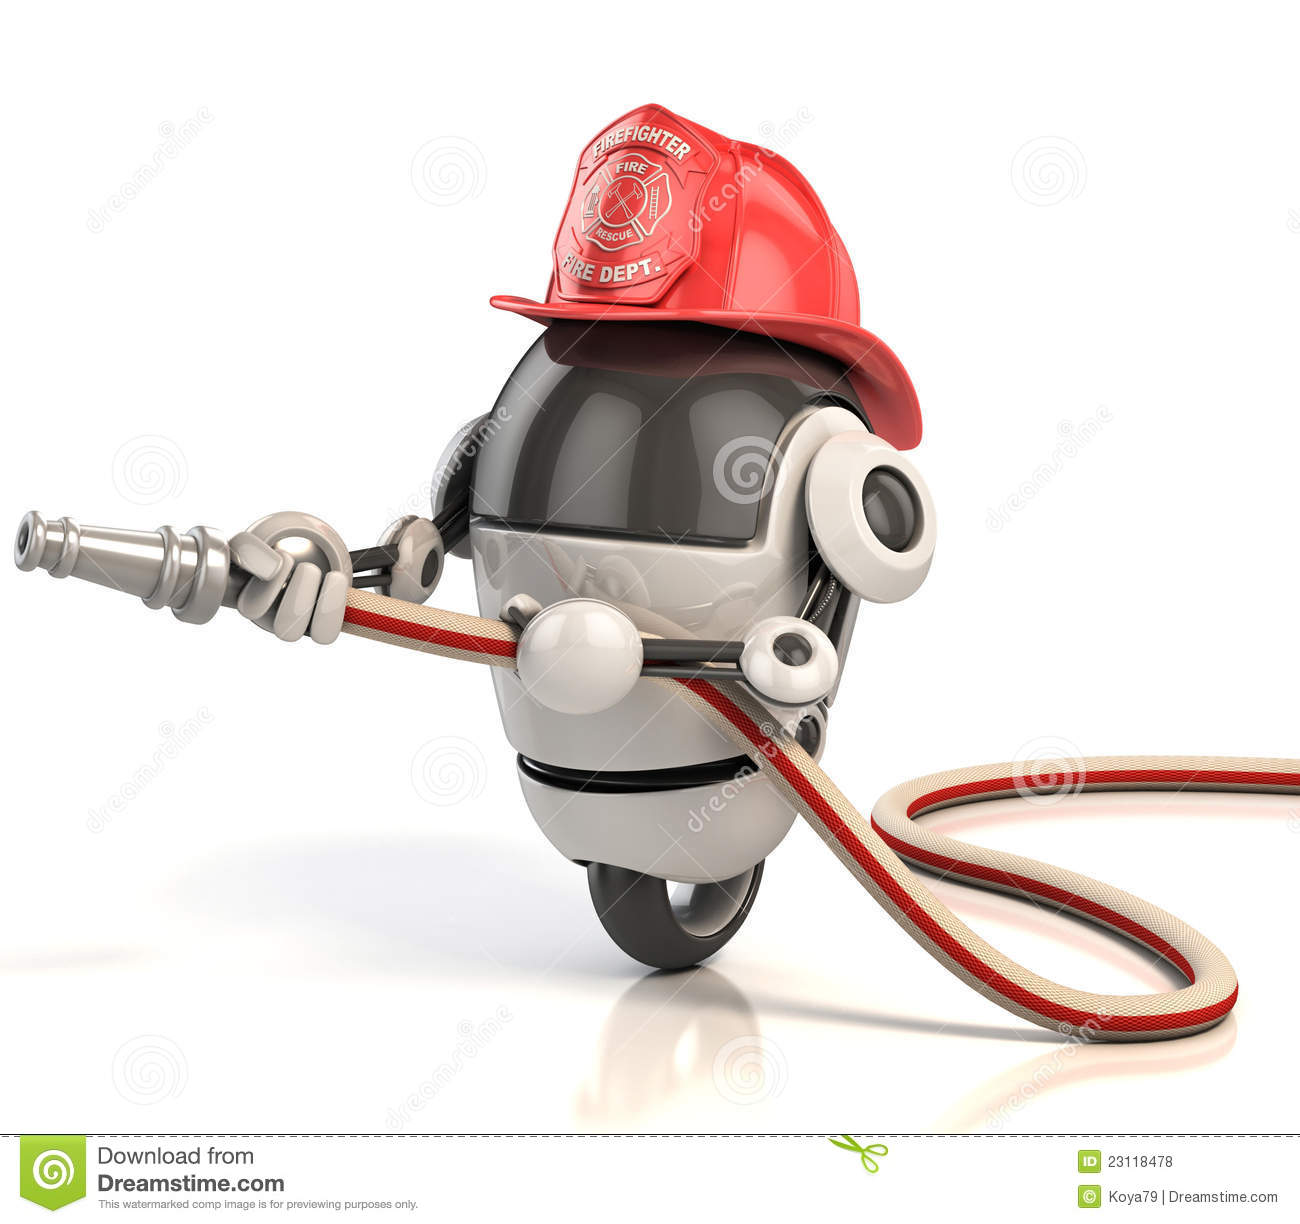
\includegraphics[width=7cm]{rapport/firebot.jpg} \\[40pt]
	\end{flushleft} 
	% séparateur 1
	{\rule{15cm}{1mm}}\vspace{7mm}
	% titres
	\begin{tabular}{p{4cm} r}
		& {\Huge {\bf \typedeprojet}} \\[20pt]
		& {\huge \nomduprojet}
	\end{tabular}\\
	% séparateur 2
	\vspace{7mm}{\rule{15cm}{1mm}}\vspace{2mm} \\
	% date
	\hfill \large \dateduprojet \hspace{2cm}
	% table des matières
	\renewcommand{\contentsname}{\LARGE \it Sommaire \hfill} % renommage de la table
	\setcounter{tocdepth}{2} % numérotation (1 pour les sections, 2 pour les sous-sections, ...)
	\tableofcontents
	\vfill
}

% auteur(s)
\author{
	\begin{tabular}{p{15cm}}
		\Large Equipe Teide 33
	\end{tabular} \\
	\hline
}

% pas de date, elle est dans le titre
\date{}

\begin{document}
\maketitle
\thispagestyle{empty} % pas de numérotation de la page de garde
\newpage

%%%%%%%%%%%%%%%%%%%%%%%%%%%%%%%%%%%%%%%%%%%%%%%%%%%%%%%%%%%%%%%%%%%%%%%%%%%%%%%%%%%%%%%%%%

\section{Plus court Chemin}

Le package chemin a pour rôle de définir les différentes classes nécessaires à la partie 3 du projet. On a choisi de créer une classe abstraite PlusCourtChemin qui permet une abstraction sur les stratégies de calculs de plus court chemin employées. Nous avons pour l'instant implémenté un seul algorithme, Dijkstra, mais il serait facile de rajouter une classe pour un autre algorithme comme A* sans avoir à modifier le reste du code.\\

Nous avons hésité entre Dijkstra et A* et finalement choisi Dijkstra car A* ne semblait pas vraiment nécessaire au problème traité. Les cartes sont relativement petites ce qui implique un nombre de noeud assez restreint, 2500 pour la plus grande carte. De plus, il serait difficile de définir une bonne heuristique puisqu'il n'y a pas d'information sur la structure "normale" d'une carte.

\subsection{Dijkstra avec un hash set}

On notera $N = n*m$, où n et m sont les dimensions de la carte, le nombre de noeuds et les complexités sont calculées en pire cas (aucun noeud inaccessible dans le graphe).
\begin{itemize}
	\item setEnsembleNoeud: Initialise le HashSet avec les noeuds sur lesquels itérer. Coût: $\theta(N)$.
	\item initDistance: Initialise le tableau de distance à $+\infty$. Coût: $\theta(N)$.
	\item getMin: Retourne le noeud non exploré le plus proche de la source. Coût: $\sum\limits_{i=0}^{N}{N-i} = \frac{N(N-1)}{2} = \theta(N^2)$.
	\item setDistanceVoisins: Met à jour les distances du tableau avec les distances des voisins. Coût: $4N-4 = \theta(N)$.\\
\end{itemize}
Complexité générale de l'algorithme: $\theta(N^2)$.\\\\
La complexité assez élevée et l'on a donc décidé d'améliorer l'algorithme avec une pile de Fibonacci ce qui permet d'atteindre la complexitée optimale en $\theta(Nlog_2(N)+4N-4)$, analyse amortie. Malheureusement, nous avons visé un peut trop haut avec une implémentation générique de la pile de Fibonacci ce qui a beaucoup compliqué le code et l'échéance approchant on a décidé de se reporter sur une solution plus simple mais qui reste très respectable: la file de priorité.\\

\subsection{Dijkstra avec une priority queue}
Il est possible d'améliorer l'algorithme en utilisant une priority queue comme structure de données. Pour cela il faut rajouter une abstraction Noeud qui contient un poids et une case, la liste est constamment ordonnée tel que l'élément de poids minimale est le premier élément de la liste, ce qui améliore la complexité de l'algorithme car la priority queue est implémentée avec un tas binaire en Java.\\
De plus, afin d'encore améliorer la rapidité de l'algorithme, nous traitons un ensemble de noeud ne contenant que la source au départ qui se remplit au fur et à mesure des détections de voisins ce qui permet de diminuer les coefficients des différentes étapes de l'algorithme.\\\\
On prend en compte le coût de chaque fonction pour la totalité de l'algorithme, pas une seule itération.
\begin{itemize}
	\item stockCarte: La nouvelle version de l'algorithme créée un tableau de noeud constitué des cases de la carte lors de la création de l'objet. Coût: $\theta(N)$.
	\item setEnsembleNoeud: Il faut initialiser tous les noeuds avec un poids à $+\infty$ et un prédecesseur à null. Coût: $\theta(N)$.
	\item getMin: La fonction à disparue il s'agit simplement de l'extraction de la tête de la file de priorité. Trouver le min de la file est en $\theta(N)$ puisqu'il s'agit de la tête, cependant il faut déterminer la nouvelle tête de file après l'extraction. Dans un tas binaire, l'opération se fait par swapping jusqu'a obtenir le min en racine. Coût: $(5N-4)log_2(N)=\theta(Nlog_2(N))$.
	\item setDistanceVoisins: On ajoute tous les noeuds du graphe dans le tas binaire. Coût: $\theta(Nlog_2(N))$ en pire cas et $\theta(N)$ en moyenne.\\
\end{itemize}
Complexité générale de l'algorithme: $\theta(Nlog_2(N))$.\\\\
La différence avec un tas de Fibonnaci ne se voit donc pas en notation $\theta$ puisque ce sont les facteurs de la complexité qui sont améliorés par cette structure de données.

\subsection{Reconstruction du chemin avec le tableau de prédecesseur}

On définit un chemin comme un hash set de Destination, à chaque noeud est associé une position et un temps de trajet pour s'y rendre en partant de la source et un temps qui est la somme des temps des sous-trajets.\\
Puisqu'il s'agit d'un hash set, il n'y a pas de notion d'ordre dans un chemin ce qui peut sembler particulier mais puisque les événements sont ajoutés avec un temps d'exécution, l'ordre n'est pas nécessaire.\\\\
\textbf{Algorithme de reconstruction de Dijkstra:} L'algorithme consiste simplement à reconstruire le chemin à partir des prédécesseurs de chaque noeud définis au cours du calcul de plus court chemin.\\
Coût: $\theta(M)$ où $M$ est la longueur du chemin en nombre de case donc $\theta(N-1)$ en pire cas.

\section{Simulation et evenements}

\verb?evenement? est un sous-package de \verb?simulation?.

\subsection{ChefPompier}

Le ChefPompier est chargé de planifier la liste des évènements. Pour cela, il possède plusieurs méthodes, qui sont appelées lorsque les évènements sont exécutés. Un cycle d'intervention d'un robot sur un incendie se déroule comme suit : 
\begin{enumerate}
	\item A chaque pas de temps, la fonction \verb?calculDeplacementExtinction? parcourt la liste des incendies, et cherche pour chacun dans la liste des robots disponibles le plus rapide à intervenir. Elle envoit ensuite ce robot à cet emplacement, donc planifie une séquence d'\verb?EvenementDeplacement? élémentaires et un évènement \verb?EvenementDeplacementFin?.
	\item Lorque ce \verb?EvenementDeplacementFin? est éxécuté, le \verb?ChefPompier? calcule le nombre de déversements maximum possible, et planifie des \verb?EvenementDeversement? et un \verb?EvenementDeversementFin?.
	\item Lorsque cet évènement \verb?EvenementDeversementFin? est éxécuté, le \verb?ChefPompier? calcule le plus court chemin pour remplir le robot, et planifie à nouveau une série \verb?EvenementDeplacement? et un autre \verb?EvenementDeplacementFin?. Si le robot n'a pas besoin de remplissage, il repasse immédiatement à 'libre' et sera affecté à un nouvel incendie au prochain pas de temps.
	\item Lorsque cet évènement \verb?EvenementDeplacementFin? est éxécuté, il planifie un \verb?EvenementRemplissage? et un \verb?EvenementRemplissageFin?.
	\item Lorsque cet évènement \verb?EvenementRemplissageFin? est éxécuté, le robot est libéré et sera affecté à un nouvel incendie au prochain pas de temps.
\end{enumerate}

NB : Dans les \verb?EvenementDeplacementFin?, un attribut sert à indiquer si c'est un évènement pour un déversement ou un remplissage, et permet au \verb?ChefPompier? d'"aiguiller" la suite de la procédure.


\subsection{ChefPompierAvance}

Cette section à été rajoutée en fin de projet et n'a malheureusement pas pu être liée au reste du projet, le code est tout de même dans l'archive mais il est impossible d'utiliser cette classe.\\

La conception d’une méthode d’ordonnancement et d’affectation des tâches a été très longue. Compte-tenu de la pluralité de nos contraintes, le problème est un problème NP-difficile. On pourrait donc le rendre aussi optimisé qu’on le souhaite, à condition de concéder du temps. \\
Après plusieurs recherches sur ce genre de problèmes, nous avons rencontré la méthode hongroise qui s’appuie essentiellement sur une approche matricielle. Grâce à des opérations élémentaires sur les lignes et les colonnes, on pouvait faire apparaître les affectations optimales. Ne pouvant, dans notre cas, pas appliquer tel quel la méthode hongroise, nous avons essayé de la réadapter. \\

Nous avons donc décidé de remplir cette matrice avec un coût  qui nous semblait pertinent : le temps. Le temps que met le robot pour se déplacer depuis sa position initiale jusqu’à l’incendie, et le temps du premier déversage qui suit. De ce fait, les contraintes liées au type de robot étaient plus ou moins bien traduites puisqu’un drone, bien que plus rapide, possède une vitesse de déversement plus lente par rapport à sa capacité.\\
A partir de ces valeurs, nous avons pu calculer la valeur minimale par ligne et la lui retrancher afin de faire apparaître un zéro ou plus. Ces zéros représentent donc des affectations réalisables mais pas forcément optimales.\\\\
En effet, la présence d'un zéro à la case (i,j) de la matrice signifie que le robot i peut être assigné à l'incendie j. Cependant, rien ne nous garantit d'avoir un seul zéro par ligne et par colonne. Il a donc fallu faire un choix arbitraire qui consiste à affecter les premiers robots que l'on trouvait (dépend donc de l'ordre de lecture de la matrice).
Dans le cas d'un robot qui n'aurait qu'un zéro, et dont ce dernier correspondrait à un incendie déjà affecté pendant ce tour de boucle, nous avons décidé d'ignorer ce robot jusqu'au prochain tour de boucle. D'un point de vue probabiliste, on peut noter la faible probabilité pour que tous les robots aient un zéro dans la même colonne.\\\\
En effet, la condition de notre boucle while dans notre méthode de $traitement$ est de continuer tant qu'il y a des incendies non éteints. La présence des deux listes $listeIncendie$ et $listeIncendieDispo$ s'explique du fait que pour éviter de créer une matrice statique qui aurait des lignes et des colonnes inutiles au fur et à mesure que l'on avancerait dans le temps. De même pour l'existence de $listeRobotDispo$.\\\\
Ainsi, $listeIncendieDispo$ nous permet de répartir le plus de robots sur le plus d'incendies différents possibles et de ne pas affecter deux robots à un même incendie si il y a encore un incendie non pris en charge (choix personnel d'optimisation). Quand cette liste est vide, cela signifie que tous les incendies sont au moins pris en charge (au plus éteints). Par conséquent, si il nous reste des robots disponibles, il nous suffit de rajouter tous les incendies non éteints à $listeIncendieDispo$ en mettant à false le booléen $enExtinction$, et ainsi éviter que des robots restent sans rien faire tant que des incendies ne sont pas effectués.\\\\
Pour la liste $listeRobotDispo$, elle nous permet de ne pas créer des lignes inutiles dans notre matrices. Il suffit à côté de mettre à jour cette liste à chaque fin de tour de boucle en rajoutant les robots qui ont fini leur tâche et ne sont donc plus occupés.

\end{document}
